\documentclass[13pt]{extreport}
\usepackage[utf8]{inputenc}
\usepackage{fullpage}
\usepackage[vietnamese,english]{babel}
\usepackage{graphicx}

\begin{document} 
\textbf{Nhóm 1 - KSTN Toán Tin K60} \\ [0.5cm]
\par \textbf{Nguyễn Anh Tú}\\
\par \textbf{Phạm Anh Tuấn}\\
\par \textbf{Trần Trọng Cường}\\[1cm]
\par \textbf{Câu 1.} Trạng thái trong bài toán là gì ? \\
Trong xử lý âm thanh, khó có thể định nghĩa được trạng thái là gì. Tuy nhiên, ta có thể phân tích rằng mỗi một cách đọc của cùng một từ khá giống nhau tuy rằng mỗi người có âm điệu và tần số riêng. Và chữ cái trong một từ có thể được hiểu như một trạng thái ẩn và âm thanh nhận được là quan sát trong mô hình Markov. Ngoài ra cũng có cách giải thích khác liên quan đến hoạt động sinh học của tai con người, tuy nhiên nhóm cảm thấy cách giải thích ban đầu là dễ hiểu và giải thích cho kết quả thu được. \\

\textbf{Câu 2.}Các overlap (chồng chất trong xử lý âm thanh) có ưu điểm và yếu điểm gì ? \\
Vì tín hiệu âm thanh thay đổi rất nhanh theo thời gian, nên chia tín hiệu âm thành các khung (frame) với mục đích rằng các frame sẽ thay đổi nhỏ và mô hình học được các thay đổi đó. Tuy nhiên nếu để frame có độ dài nhỏ thì ko có đủ thông tin để thực hiên MFCC còn để frame lớn thì âm thanh lại thay đổi nhanh. Vì vậy sử dụng các frame vừa đủ và cho chúng chồng chất lên nhau là cần thiết để vừa có thể có một frame đủ rộng để thực hiện MFCC và các frame gần nhau không thay đổi quá nhiều.

Nhược điểm của việc nhiều overlap thì khá rõ ràng khi overlap (thông thường từ 25\% - 50\%) nghĩa là nhiều frame trong tín hiệu âm thanh và như vậy số lượng tính toán lớn hơn nhiều. \\

\textbf{Câu 3.}Ngoài MFCC còn phương pháp gì để xứ lý âm thanh hay không ? \\
Ngoài MFCC, còn có các phương pháp khác như là LPC (Linear Predictive Encoding) và FFT(Fast Fourier Transform), tuy nhiên các phương pháp mà nhóm tìm hiểu được đều dựa trên biến đổi Fourier. \\

\textbf{Câu 4.} Hàm hợp lí là gì ? \\
Giả sử ta có một mẫu dữ liệu $O = {O^1, O^2, ..., O^T}$ và gọi $\lambda$ là tham số của một mô hình nào đó. Khi ấy, hàm hợp lí đánh giá độ phụ hợp của việc mô hình với tham số $\lambda$ sinh ra mẫu dữ liệu $O$
$$P(O | \lambda)$$

\textbf{Câu 5.} Gaussian được trộn vào tín hiệu gì ? Lý do tại sao trộn ? \\
Mô hình Gaussian hỗn hợp được sử dụng để xấp xỉ hàm mật độ của biến đầu ra ở mỗi trạng thái. Nói gắn gọn thì với một mẫu dữ liệu $O = {x^1, x^2, ..., x^N}$, mô hình GMM sẽ tìm các tham số $c_j, \mu_j, \Sigma_j$ để cực đại hàm hợp lý của
$$ p(x) = \sum_{k = 1}^N c_j \mathcal{N}(x | \mu_j, \Sigma_j)$$
Đối với bài toán xử lý âm thanh thì các $x^i$ ở đây là các vector ứng với mỗi frame sau khi được xử lý sử dụng MFCC. Lý do xử dụng mô hình này là vì lý thuyết đã chức minh được mô hình này với số lượng phân phối chuẩn hợp lí có thể xấp xỉ mọi hàm mật độ. \\

\textbf{Câu 6.} Số lượng trạng thái của âm thanh là gì ? \\
Như đã trả lời ở câu hỏi 1, cách hiểu đúng trạng thái ở đây là gì có nhiều ý kiến khác nhau, và vì thế nên số trạng thái khó xác định. Để chọn ra trong mô hinh có bao nhiêu trạng thái nhóm làm 2 công việc, thứ nhất là chiếu các vector thu được từ phương pháp MFCC lên mặt phẳng và xem xét tính phân cụm của chúng và chạy mô hình trên nhiều số lượng trạng thái khác nhau mà xem xét kết quả. Nhận xét số lượng trạng thái của mô hình khá giống với việc chọn số neural trong lớp embedding của mạng neural. \\

\textbf{Câu 7, 8.} Tính mới của đồ án và đóng góp của tác giả. \\
Thứ nhất trong bài báo cáo này, nhóm đã sử dụng mô hình HMM để nhận diện Tiếng Việt. Mặc dù đã có những nghiên cứu cùng đề tài đó nhưng hầu hết chỉ nói đến việc xử lý âm thanh như thế nào. Công việc của nhóm đã tổng hợp được lý thuyết ứng dụng của Markov ẩn vào nhận diện giọng nói. Trong nhiều tài liệu, khi cập nhật tham số đới với trường hợp có nhiều dãy quan sát, thường làm chạy giải thuật Baum-Welch tuần tự các quan sát, nhưng cách làm này không làm tối ưu hàm $\prod P(O^i | \lambda) $ mà chỉ tìm nghiệm tối ưu địa phương cho dãy quan sát được chạy cuối cùng. Bên cạnh đó đối với tiêng việt,  nhóm khi phân tích dữ liệu tự thu thập được đã đưa ra được số trạng thái ẩn, số phân phối gaussian, độ dài khung và đồ đè của khung tin hiệu để thu được mô hình nhận diện giọng nói đặt được kết quả cao. \\

\textbf{Câu 9.} Kết quả đánh giá mô hình \\
Kết quả đánh giá mô hình được miêu tả trong chương cuối của báo cáo. \\

\textbf{Câu 10.} Tại sao GMM lại liên quan đến phân cụm ? Phân cụm bao nhiêu lớp ? \\
Công thức trong hai bước E và M đã được ghi trong bài báo cáo. Hình sau minh họa cho tính phân cụm của GMM, với L là số lần thực hiện lặp 2 bươc E và M. Hình (a) khợi tạo 2 phân phối chuẩn, hình (b) thể hiện khi tính bươc E,, các hình còn lại ứng với số vòng lặp 2 bước E-M.
\begin{center}
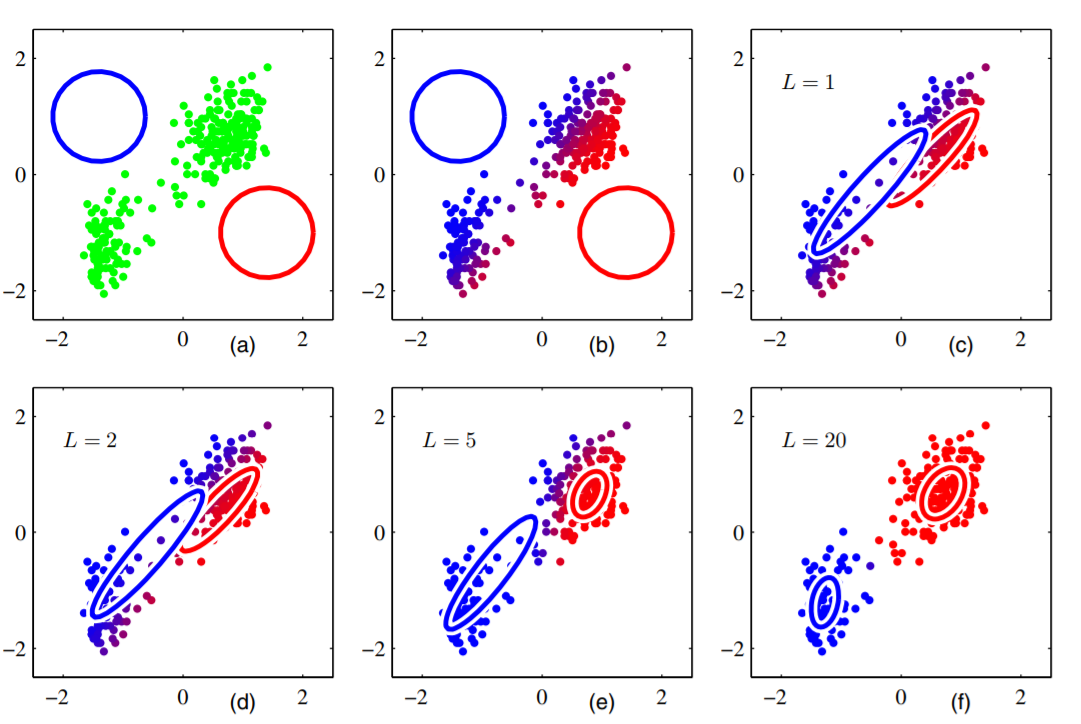
\includegraphics[scale=0.7]{gmm_exp.PNG}
\end{center}
Đặc biệt, khi khởi tạo ma trận hiệp phương sai của các phân phối chuẩn là ma trận đơn vi thì ta kến quả nhận được các kì vọng chính là các tâm sinh ra bởi thuật toán K-means.Còn số lượng phân cụm chính bằng số phân phối chuẩn trong mô hình GMM.


\end{document}